For the task of classification, in which observations are globally known it is not necessary to model joint probability distribution over all possible outputs and observed values. Instead, it is possible to model conditional distribution $P(Y|X)$, which is a distribution of output variables on condition that input variables take an observed form.  A type of Markov Random Fields that take this approach is called Conditional Random Field \cite{crf_lafferty}. They can be viewed as undirected graphical models, which represent both observations, and output labels. With the use of factor graphs, factorisation of a probability distribution can be modelled. Those graphs contain two different types of variables, inputs and outputs \cite{crf_sutton}. The first ones are observed input variables denoted as $x$ from the input domain $X$, which is dependent on an application. For semantic image segmentation, $x$ would be a single image from the set of all available images, represented in terms of a feature vector containing observed properties of an image such as pixel intensity, texture, or colour histograms in terms of numerical values. A great advantage of Conditional Random Fields is that they can involve a large variety of different features. Input variable nodes are connected via factors to the second type of nodes, which are known as hidden nodes, as they cannot be directly obtained from an observed object. Those nodes represent output variables $y$ from the output domain $Y$ being for example labels assigned to pixels from a set of all possible labels. They are as well connected with each other with the use of factors making it possible to take into consideration relations between neighbouring entities like pixels in an image. Figure \ref{fig:factor_graph} presents how such a graph can be constructed on an example of an image with size $3\times3$ pixels.
\begin{figure}[h]
    \centering
    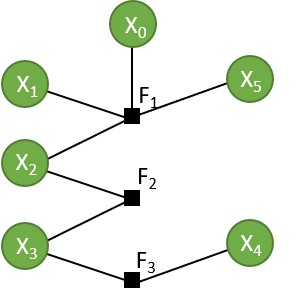
\includegraphics[width=0.5\textwidth]{factor_graph}
    \caption{Factor graph representing an image $3\times3$ pixels }
     \label{fig:factor_graph}
\end{figure}
On the graph, blue circles represent input nodes with observed variables, and green circles a hidden layer of output nodes. Factors, which join each output node to the corresponding input node as well as every neighbouring output nodes are marked as black squares. Between each pair factor – node there is an edge presented as a line, which connects them. This is the simplest type of the graph, though it is also possible to introduce other dependencies for example between an output node and observation nodes related to neighbouring output nodes. 
Such a graph model conditional distribution $P(Y|X)$ which can be expressed in terms of energy of a factor. Given the fact that there are two types of factors, one connecting an input node to an output node and the other one between every pair of output nodes, energy is defined differently depending on a factor kind. For the latter type, a pairwise potential is used, which reflect a relation between labels of neighbouring output nodes. It introduces a penalty if neighbouring output nodes have a different label by assigning high energy values to such configurations and as a result lower probability of their occurrence. For modelling energy connected with factors joining input and output nodes a unary potential is introduced. It models a relationship between observed features and a predicted label. It should assign high values of energy for a wrong label assigned to an output node of a given input node and low energy values for proper assignments. It is used to promote a situation in which two nodes which are similar in terms of a feature vector have the same label. Hence, an energy of a whole factor graph can be described with the following formula with each variable node from a variable set $V$ denoted as $i$ and each neighbour $j$ of the node $i$.
\begin{equation}
    E(Y=y,X=x)=\sum_{i\in V}{E_1}({y_i},{x_i}) + \sum_{i,j\in V}{E_2}({y_i},{y_j})
\end{equation}
In order to define the factor energy, it is required to perform parametrisation with a set of weights w so that it possible to map observed input values to outputs. Then, energy is dependent on three types of variables, inputs, outputs, and parameters \cite{inference_crf}.

There are multiple ways of defining unary potentials tough the goal is always to represent relations between a feature vector of a given input node and all possible outputs. In semantic image segmentation, this term predicts label of a given pixel or region basing on some observed features of this part of an image. In the most basic form, local energy is specified by a linear function describing a relation between chosen parameters in a form of a weight vector w and a feature vector $\varphi$ \cite{Nowozin}, as in formula \ref{energy_basic}.
\begin{equation}
    \label{energy_basic}
    E_1(y_i,x_i)=\left \langle w(y_i),\varphi_i(x_i) \right \rangle
\end{equation}
A weight vector is dependent on an output label $y$ as a separate weight is associated with each feature for every possible class.

When it comes to defining pairwise potential, the simplest, and yet a popular method is to introduce two parameters which directly reflect an energy. If two neighbouring nodes have the same label than an energy of the factor between them will be equal to weight $w_1$, if not $w_2$.
\begin{equation}
    E_2(y_i,y_j)=\begin{Bmatrix}
     w_1 & y_i=y_j \\ 
     w_2 & y_i \neq y_j
    \end{Bmatrix}
\end{equation}
A more detailed explanation on how an energy function can be expressed will be provided in section \ref{sec:energy} \nameref{sec:energy}. 

Having specified how an exemplary energy function can be created, in order to make predictions about an unobserved object, it is necessary to find such a combination of output variables in a factor graph that will give the lowest energy as this would be a most probable setting. However, it is computationally intractable to calculate graph energy for every possible label configuration especially for problems involving large data structures. On an example of semantic image segmentation, even for a small problem of segmenting an image with size $100\times100$ pixels into two classes, it would require to calculate energy for $2^{100\times100}$ combinations and real-life problems are much more complicated. Because of this, in most cases, it is impossible to obtain an exact solution for classification problems based on factor graph energy. Though, it is possible to approximate a solution.